% This is based on the LLNCS.DEM the demonstration file of
% the LaTeX macro package from Springer-Verlag
% for Lecture Notes in Computer Science,
% version 2.4 for LaTeX2e as of 16. April 2010
%
% See http://www.springer.com/computer/lncs/lncs+authors?SGWID=0-40209-0-0-0
% for the full guidelines.
%

\documentclass[a4paper]{article}


\usepackage{color}
\usepackage{float}

\usepackage{booktabs}
\usepackage[dvipsnames]{xcolor}
\usepackage{tikz}

\usepackage{amsmath}
\usepackage{amssymb}
%% Language and font encodings
\usepackage[english]{babel}
\usepackage[utf8x]{inputenc}
\usepackage{graphicx}
\usepackage[colorinlistoftodos]{todonotes}
\usepackage[colorlinks=true, allcolors=blue]{hyperref}

\usepackage[T1]{fontenc}

\definecolor{codegreen}{rgb}{0,0.6,0}
\definecolor{codegray}{rgb}{0.5,0.5,0.5}
\definecolor{codepurple}{rgb}{0.58,0,0.82}
\definecolor{backcolour}{rgb}{0.95,0.95,0.92}


\newcommand{\dummyfigure}{\tikz \fill [NavyBlue] (0,0) rectangle node [black] {Figure} (2,2);}


\usepackage[a4paper,top=3cm,bottom=2cm,left=3cm,right=3cm,marginparwidth=1.75cm]{geometry}

 
%\lstdefinestyle{mystyle}{
%    backgroundcolor=\color{backcolour},   
%    commentstyle=\color{codegreen},
%    keywordstyle=\color{magenta},
%    numberstyle=\tiny\color{codegray},
%    stringstyle=\color{codepurple},
%    basicstyle=\footnotesize,
%    breakatwhitespace=false,         
%    breaklines=true,                 
%    captionpos=b,                    
%    keepspaces=true,                 
%    numbers=left,                    
%    numbersep=5pt,                  
%    showspaces=false,                
%    showstringspaces=false,
%    showtabs=false,                  
%}
 
%\lstset{style=mystyle}



\begin{document}

\title{Image Caption Generation with CNN-RNN, Soft Attention and Top-Down Bottom-Up Attention}
%
\author{Saurabh Kulshreshtha, Daniel DiTommaso, Robin Bhattacharya}
%\institute{University of Massachusetts Lowell}

\maketitle              % typeset the title of the contribution

\begin{abstract}
\noindent One of the most important problems in computer vision is describing images. Although image captions can be ambiguous, given the possibilities of the descriptions is large - there has been a fair amount of research and progress on the this topic so far. Generating captions involves two important aspects, i.e., a representation of the images and a representation of the caption. Images are represented best with Convolutional Neural Networks and improvements thereof and captions are best generated by some form of Recurrent Neural Networks. They can be naively combined which is first model we study, or combined in a more holistic manner using attention which is the other two models we study. Here we explore three popular network architectures, Show and Tell\cite{DBLP:journals/corr/VinyalsTBE14} and Show, Attend and Tell\cite{DBLP:journals/corr/XuBKCCSZB15} and very recent work Top-Down and Bottom-Up Attention\cite{DBLP:journals/corr/AndersonHBTJGZ17}, all three have been state-of-the-art when first released. These models build on top of each other adding better representational capacities and improving the results and power of the models but also increase in complexity and become harder to train. All the models were able to describe the images with very high precision.
\end{abstract}
\section{Goal}
Image captioning is the process of generating a text description of an image. Its important but a challenging task; few applications of image captioning include virtual assistants, support for the disabled, different indexing tools and indexing of images.  Our goal in this paper is to use different architectures to obtain incrementally better representations of both the image and caption generation subsystem which generates the final captions.

\section{Introduction}
For a human, a quick glance is sufficient for it to describe an image or a scene in a detailed manner. Historically, this has been difficult to achieve with machines. Previously, some pioneering work in visual recognition has been done but limited to fixed visual categories. Although impressive, these models were limited to hard-coded visual concepts and other sentence templates, which is vastly limiting when we compare it to a human eye. However, things have started changing over time.
\\
\\
\noindent In  recent years the amount of data available has increased in leaps and bounds. As a result, the approach towards handling the problem has changed drastically. Along with increasing data we also have the rise of Deep Neural Networks which facilitates the change in approach. These new techniques have largely been based on recurrent neural networks(RNNs) powered by Long Short Term Memory(LSTM) which takes care of the vanishing or exploding gradient problems. Owing to the ability of LSTMs to memorize long term dependencies through a memory cell, it becomes a go-to network for language-vision tasks like image captioning, visual answering, situation recognition, visual dialog etc\cite{DBLP:journals/corr/abs-1711-09151}. Unlike Convolutional Neural Networks(CNN) LSTMs require sequential processing and storage due to back-propagation during training time. So, CNNs and LSTMs were not really matched up for vision-language tasks until very recently.
\\
\\
\noindent With the recent success of CNNs with different sequence to sequence, the image captioning approach has changed. We try the same new approach here, starting with the original paper "Show and Tell". Just like machine translation architecture where we use an RNN, here we use a CNN as an encoder where given an image it produces a rich fixed-length vector representation of the image. This is where the image is "encoded". Now we feed the representation from the last hidden layer of the CNN to the "decoder" RNN which will generate a caption of the image.
\\
\\
\noindent Here our aim is to try out different architectures of CNNs in the encoder layer to see how well those fixed-length representations generated from these various architectures determine the quality of the captions generated when trained on those representations. We implement an end to end system for this architecture. Starting from Show and tell we also implement the version with attention or Show Attend and Tell, and the Top down and Bottom Up Attention approach for Image captioning.  

\section{Background}
As of late there have been strong experiments on image and video captioning owing to the change of methodology. Earlier systems of and-or-graphs were used, which required conversion to human interpretable natural language using rule based systems. These systems were brittle and heavily based on humans. The current approach is drastically different, for example Show and Tell \cite{DBLP:journals/corr/VinyalsTBE14} and others. Here a neural and a probabilistic framework is used with a powerful sequence model. These models have the capability of producing state of the art results by maximizing the probability of the input sequence given in an "end to end" fashion. The general approach involves encoding the input image into a fixed dimensional vector, which then is fed to the recurrent neural network (RNN) for it to "decode" \par
The usual method involves increasing the probability of the correct caption using the following formula:\par

$\theta$ $=$ arg $max_\theta$ $\Sigma_(I,S_)$ log p(S$|$I; $\theta$) \par \cite{DBLP:journals/corr/VinyalsTBE14}
Here theta are the parameters, I is the image and S is the transcriptions.  \par
Another approach that has been used in the recent past is CNNs with attention mechanism in both image captioning and VQA tasks. Attention captioning models either uses edge boxes \cite{zitnick2014edge} or spatial transformer networks \cite{DBLP:journals/corr/JaderbergSZK15} which are processed using an attention model which are paired using three bi-linear attention models. There are two particular kind of methods; namely top down and bottom up attention mechanism. The Bottom up approach involves using faster R-CNN \cite{ren2015faster}which identifies instances of objects with certain classes and bounds them with a rectangle. The top down approach on the other hand involves characterizing the first layer of the LSTM which produces captions as the top-down visual attention model and the second layer as the language model, Thus producing state of the art results. Although these are the models which have been implemented before, our goal here is to implement these models with a newer framework.

\section{Approach}
We work towards the implementation and evaluation of three at the time state-of-art networks. Each of these have built on the success of the previous one taking the best elements and incorporating new representational tools. Starting with Show and Tell, the caption generation subsystem is based on a vanilla recurrent architecture, which incorporates the recent advances in computer vision and machine translation. This model is built to maximize the probability of the target description sentence on a given training image per word assuming the previous predicted words were all equivalent to the target description (teacher forcing).\cite{DBLP:journals/corr/VinyalsTBE14} Next, we work towards implementation and evaluation of Show, Attend and Tell where a model is trained in a deterministic manner using standard backpropagation techniques.\cite{DBLP:journals/corr/XuBKCCSZB15} Lastly, we work towards implementing and evaluation of an approach which combines the top-down and bottom-up attention mechanism - which allows attention to be calculated at the level of objects and other salient image regions at two levels, first, a bottom up approach to detect objects and next top down attention to attend to these variably sized objects and generation of captions. \cite{DBLP:journals/corr/AndersonHBTJGZ17} Here we use one of the benchmark datasets; Flickr8k as they are comparatively smaller in size and are faster to train. 
\subsection{Show and Tell Model}
As we said with the recent success of language translation model, with end to end sequences, there has been implementation of CNN in the encoder part to obtain a representation of images. It uses the following formula.\par
\begin{center}
$\theta$ $=$ arg $max_\theta$ $\Sigma_(I,S_)$ log p(S$|$I; $\theta$)
\end{center} \par \cite{DBLP:journals/corr/VinyalsTBE14}
where $\theta$ are the parameters of the model, I are the images of the model and S are the transcriptions. Since it is obvious that the length of S is unbounded or varied we could use chain rule to obtain the joint probability. \par
\begin{center}log p(S$|$I) = $\Sigma$ log p(S of t given I, from S of 0 to t-1)\end{center}
dependency on $\theta$ is dropped as it is more convenient. So at any given point during training time we have a pair as (S,I) and we implement gradient descent algorithm on it to reduce its loss. LSTM based sentence generation is used as it is better equipped to deal with vanishing and exploding gradient problems. The overall architecture of the model is better understood through this picture above; Figure 1. \cite{DBLP:journals/corr/VinyalsTBE14}

\begin{figure}
\centering
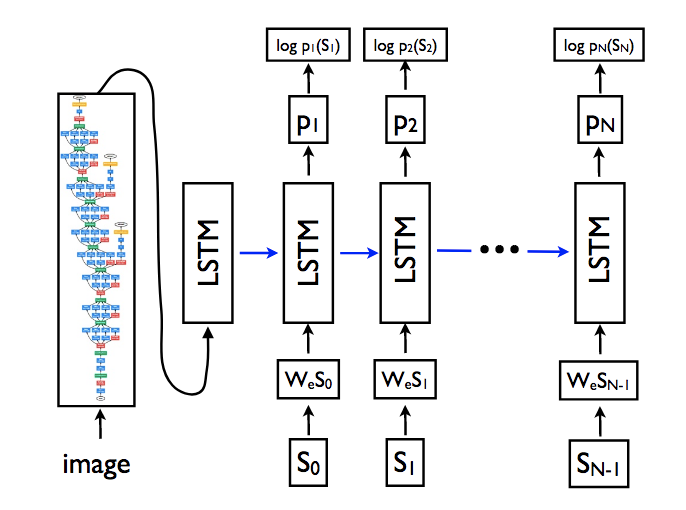
\includegraphics[width=0.4\textwidth]{sc1.png}
\caption{\label{fig:arch}Diagram representing the architecture of Show and Tell.}
\end{figure}

\subsection{Show, Attend and Tell}
When there are a large number of entities in a scene it becomes difficult for a simple model such as RNN to take into account the various interactions betweens these objects and come up with a exhaustive and complete description of the image - instead the simpler models tend to gloss over. Humans on the other hand tend to focus on parts of the image, paying attention and checking interactions between the important objects in the scene as we go on describing the image. A similar attention mechanism has been proposed to mimic human behavior\cite{DBLP:journals/corr/XuBKCCSZB15}. This attention mechanism allows only a certain part of the features to be input into the RNN. At each step, the salient region of the image is determined and is fed into the RNN instead of using features from the whole image. The determination of which spatial region will be chosen depends on the previous words that have been generated by the RNN already. The recurrent network now only gets a focused view from the image and predicts the word relevant to that region. New generated words are coherent within the region but not in the description being generated if the prior words generated are not a parameter to the attention mechanism.\\
\\
Mathematically, we are trying to replace the image x in LSTM model,
\begin{figure}[H]
\centering
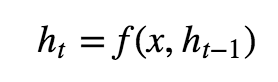
\includegraphics[width=0.2\textwidth]{1.png}
\end{figure}
\noindent with an attention module attention:
\begin{figure}[H]
\centering
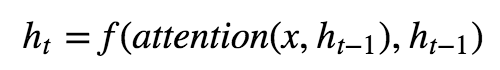
\includegraphics[width=0.35\textwidth]{2.png}
\end{figure}
\noindent The attention module has 2 inputs:\\
1. A context\\
2. Image features in each localized areas.\\
\\
For the context, we use the hidden state $h_t−1$ from the previous time step. In a LSTM system, we process an image with a CNN and use one of the fully connected layer output as input features $x$ to the LSTM.\\
\begin{figure}[H]
\centering
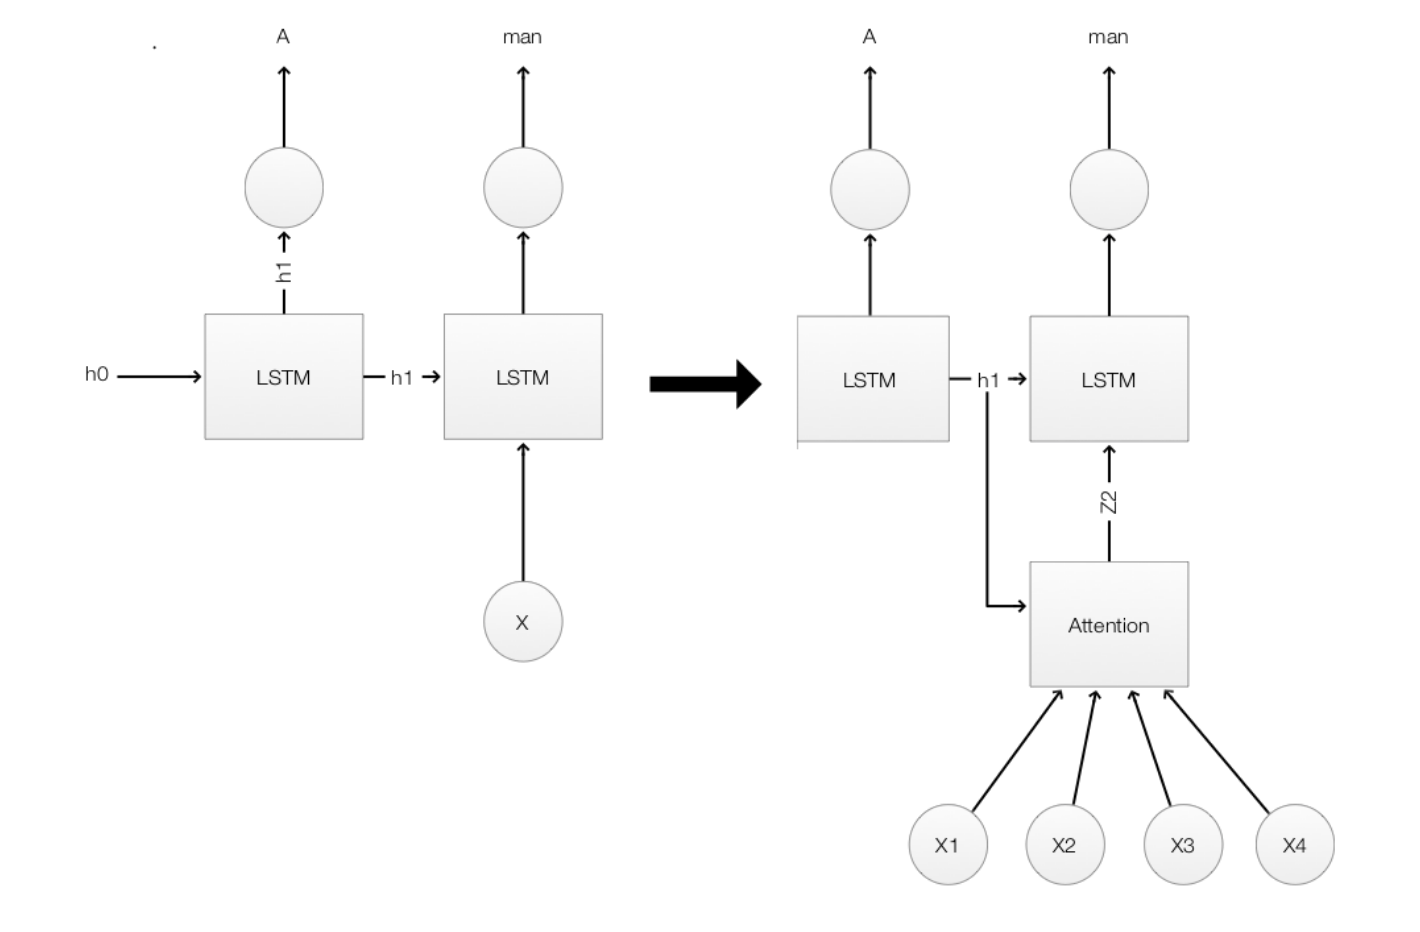
\includegraphics[width=1\textwidth]{3.png}
\end{figure}

\begin{figure}[H]
\centering
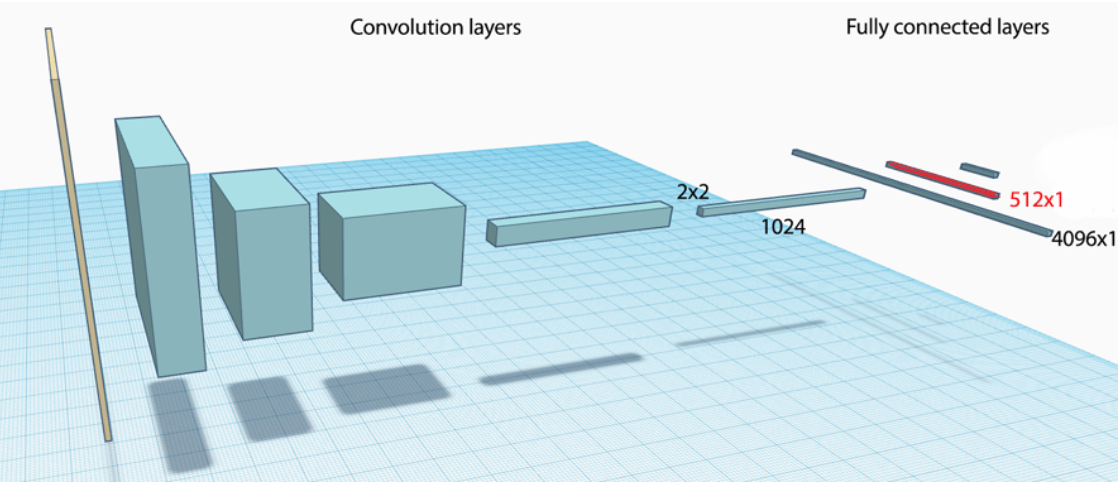
\includegraphics[width=1\textwidth]{4.png}
\end{figure}

\noindent Nevertheless, this is not adequate for an attention model since spatial information has been lost. Instead, we use the feature maps of one of the convolution layer which spatial information is still preserved.

\begin{figure}[H]
\centering
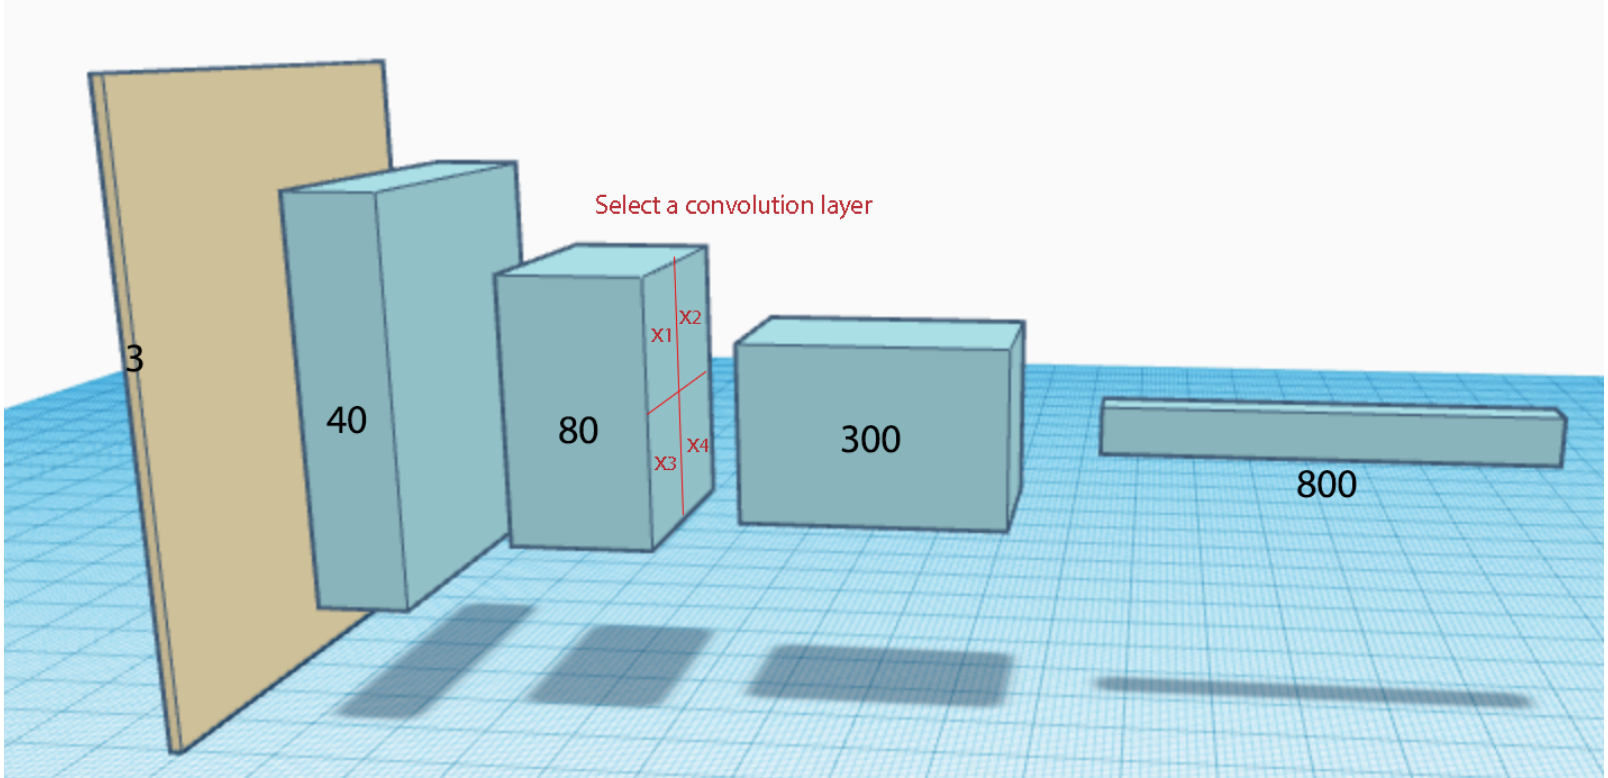
\includegraphics[width=0.7\textwidth]{5.png}
\end{figure}
\noindent Here, the feature maps in the second convolution layers are divided into 4 which closely resemble the top right and left and the bottom right and left of the original pictures. We replace the LSTM input $x$ with an attention module. The attention module takes the context $h_t−1$ and 4 spatial regions $(x1,x2,x3,x4)$ from the CNN to compute the new image features used by the LSTM.
\begin{figure}[H]
\centering
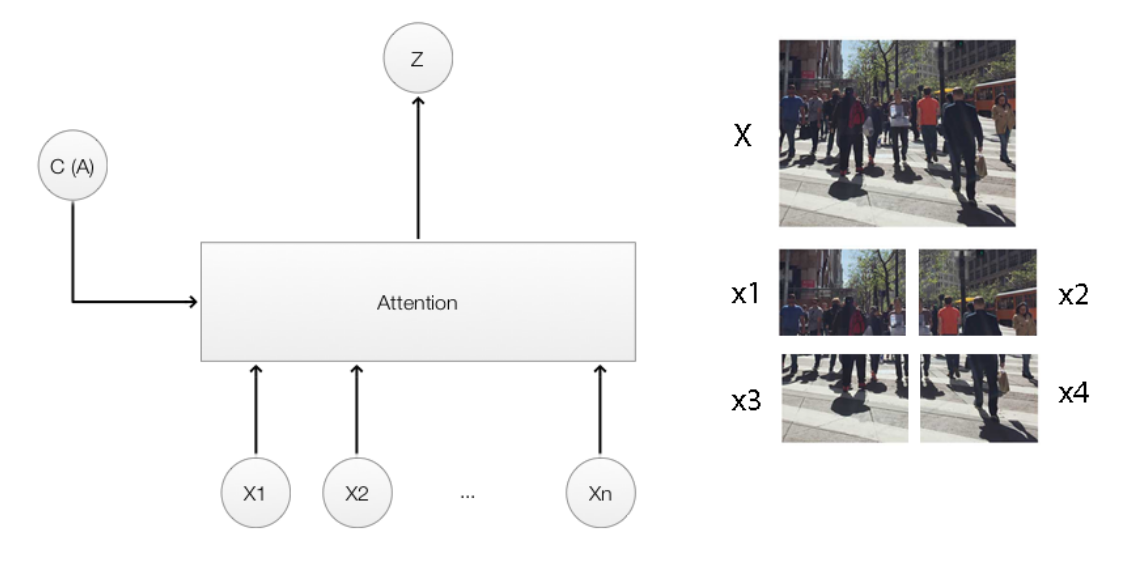
\includegraphics[width=1\textwidth]{6.png}
\end{figure}
The following is the complete flow of the LSTM model using attentions.
\begin{figure}[H]
\centering
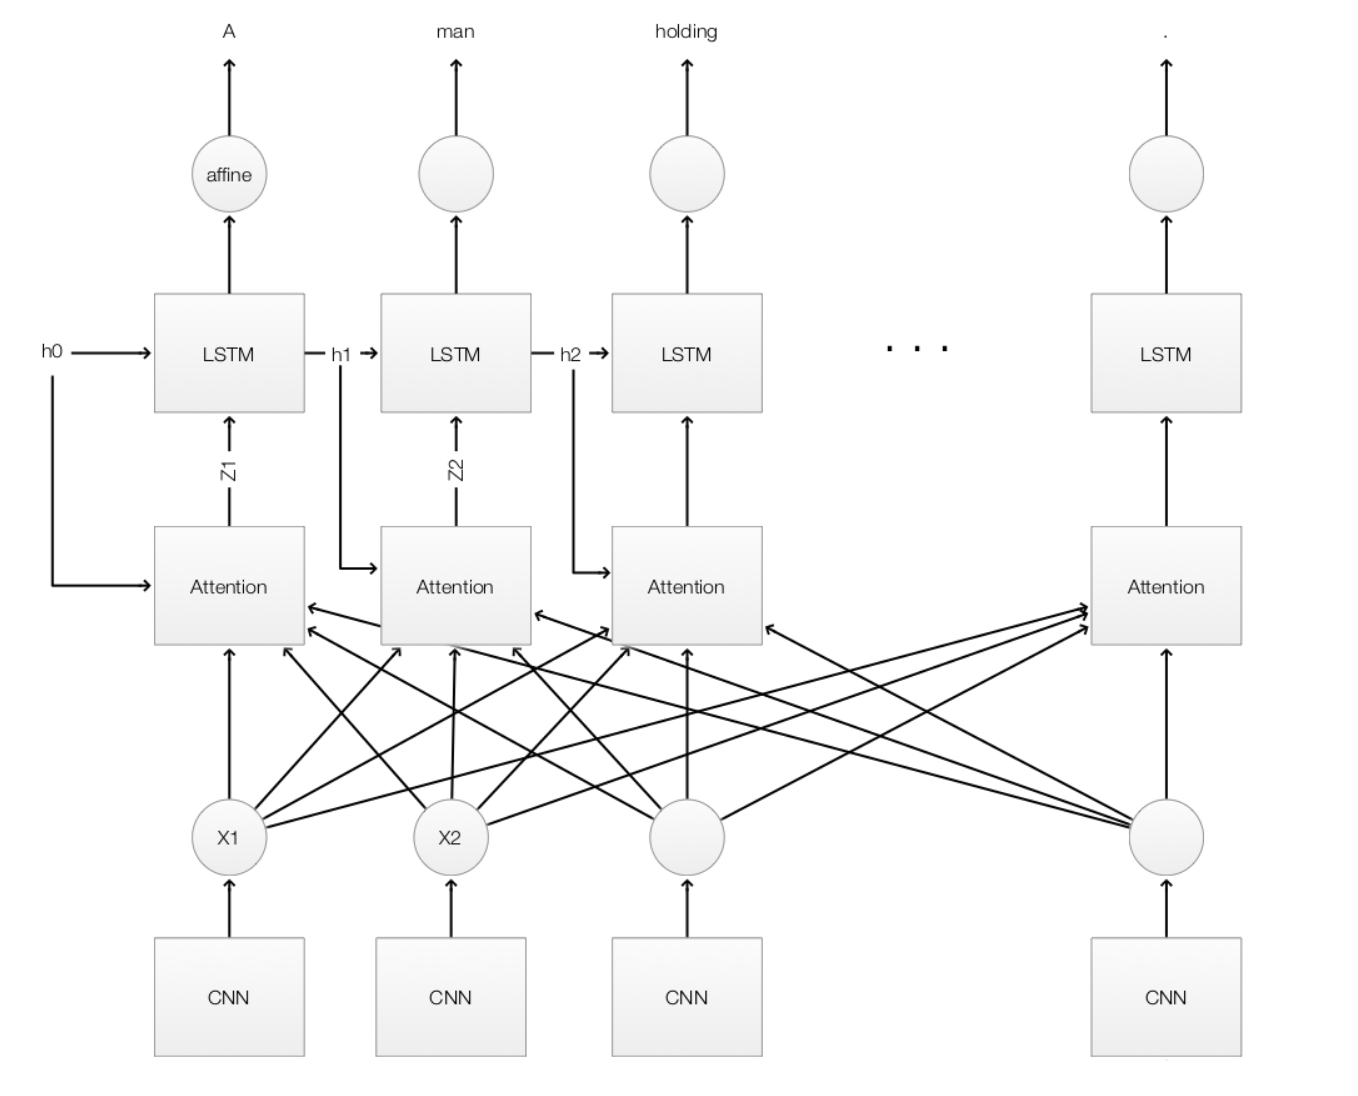
\includegraphics[width=0.7\textwidth]{7.png}
\end{figure}
\subsubsection{Soft Attention}
We implement attention with soft attention. In soft attention, instead of using the image x as an input to the LSTM, we input weighted image features accounted for attention. Before going into details, we can visualize the weighted features to illustrate the difference. Areas with higher attention are brighter in the picture.
\begin{figure}[H]
\centering
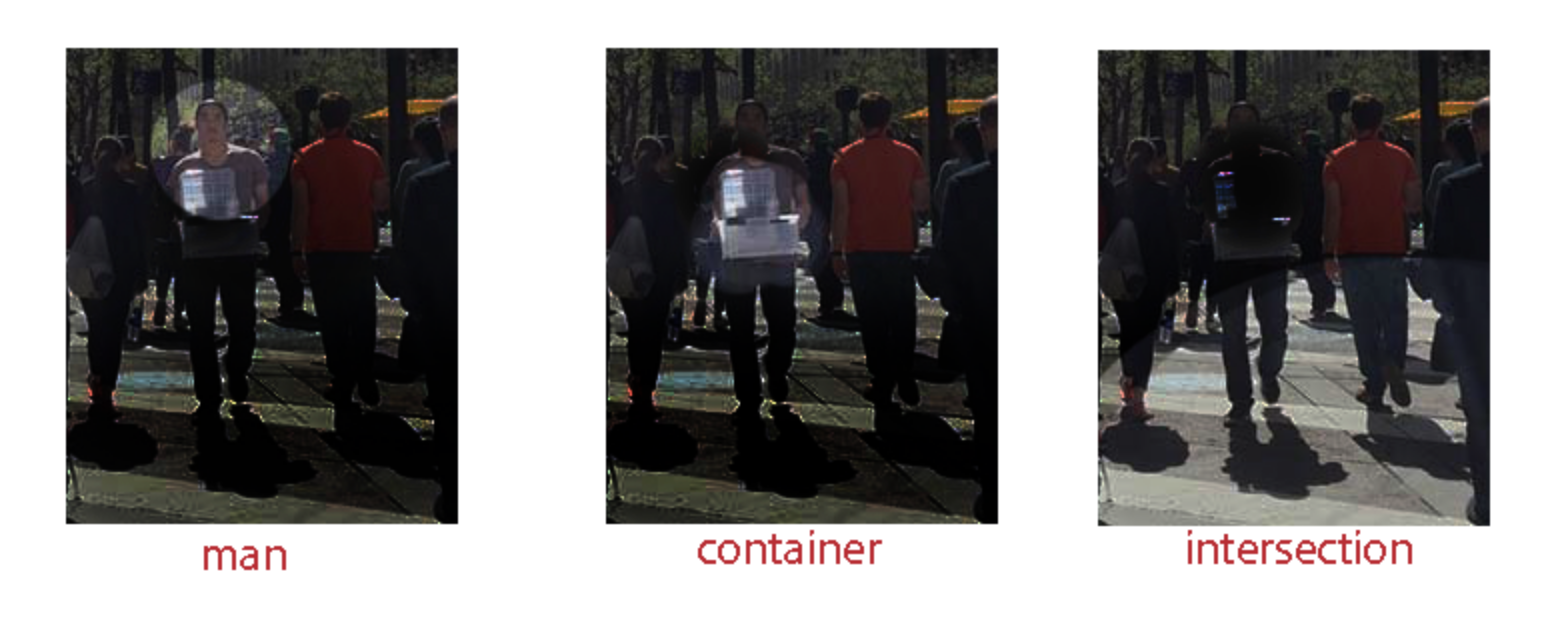
\includegraphics[width=0.8\textwidth]{man.png}
\end{figure}

\noindent This picture visualizes the weighted features to the LSTM and the word it predicted. Soft attention discredits irrelevant areas by multiplying the corresponding features map with a low weight. Accordingly, high attention area keeps the original value while low attention areas get closer to 0 (become dark in the visualization). With the context of “A man holding a couple plastic”, the attention module creates a new feature map with all areas darkened except the plastic container area. With more focused information, the LSTM makes a better prediction (the word “container”).\\
\\
Let’s show how to compute the weighted features for the LSTM. $x_1$,$x_2$,$x_3$ and $x_4$ each covers a sub-section of an image. To compute a score $s_i$ to measure how much attention for $x_i$, we use (with the context $C=h_t−1$):

\begin{figure}[H]
\centering
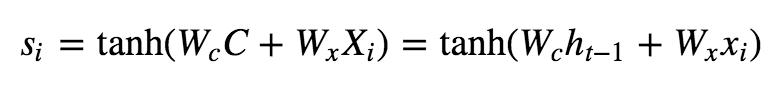
\includegraphics[width=0.5\textwidth]{8.png}
\end{figure}
\noindent We pass $s_i$ to a $softmax$ for normalization to compute the weight $\alpha_i$.
\begin{figure}[H]
\centering
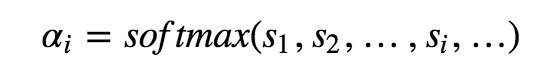
\includegraphics[width=0.4\textwidth]{9.png}
\end{figure}
\noindent With softmax, $\alpha_i$ adds up to 1, and we use it to compute a weighted average for $x_1,x_2,x_3$ and $x_4$.
\begin{figure}[H]
\centering
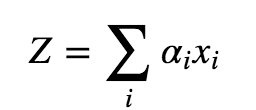
\includegraphics[width=0.18\textwidth]{10.png}
\end{figure}

\noindent Finally, we use $Z$ to replace $x$ as the LSTM input.

\begin{figure}[H]
\centering
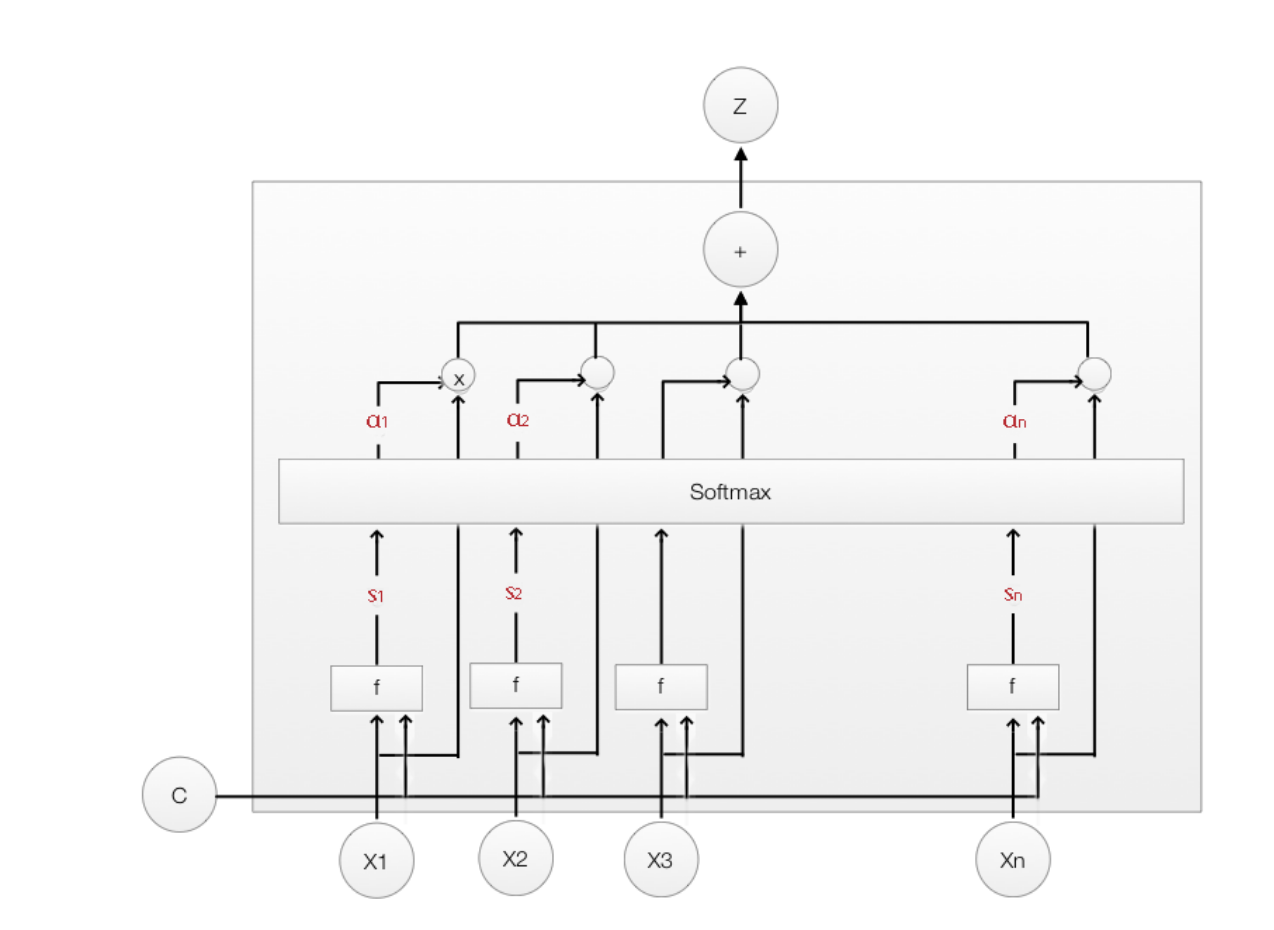
\includegraphics[width=0.75\textwidth]{11.png}
\end{figure}

\subsection{Top Down and Bottom up Attention}
Given an image $I$, this captioning model takes as input a possibly variably-sized set of $k$ image features generated by an R-CNN(Region-based Convolutional Neural Network), $V = {v_1, ..., v_k}$, $v_i \in R^D$, such that each image feature encodes a salient region of the image.\\
\noindent The spatial image features V can be variously defined as the output of  the bottom-up attention model. We summarize the approach to implementing a bottom-up attention model in Section 4.3.1, and the architecture of the image captioning model in Section 4.3.2. Both of which come from the original work. \cite{DBLP:journals/corr/AndersonHBTJGZ17}
\\

\subsubsection{Bottom-Up Attention}
The spatial regions are defined in terms of
bounding boxes and implement bottom-up attention using
Faster R-CNN \cite{ren2015faster}. Faster R-CNN is an object detection
model designed to identify instances of objects belonging
to certain classes and localize them with bounding boxes.
\\

\noindent 
Faster R-CNN detects objects in two stages. The first
stage, described as a Region Proposal Network (RPN), predicts
object proposals. Features are processed using a smaller CNN network. The network predicts a score for each proposal and realizes boxes of various scales. An intersection-over-union(IoU) is the accuracy of an object detection model. Using an IoU threshold the best proposals are used for input to the second stage. The second stage is comprised of extracting a feature map for each region. The final output of the model is a softmax distribution of class labels and bounding box refinements of every proposal.
\\

\noindent In this work, Faster R-CNN is combined with ResNet \cite{DBLP:journals/corr/HeZRS15}. The features for each image are calculated by taking the model output and using a process known as non-maximum supression(NMS). NMS essentially combines all of the detected regions that belong to the same object. All detected regions which surpass a confidence threshold are passed through a mean-pooled convolution. This process decides a feature pertains to a general region, which allows the model to focus on 'hard' attention points. This reduces the overall number of features for a given region.
\\

\subsubsection{Captioning Model}

Using the set of image features generated above the model processes futher using a top-down attention model. This model weights each feature for caption generation utilizing the caption fragment. This is in essence a two stage LSTM model. The two LSTMs work in conjuction to map which words in the caption pertain to which features of the image. 
\\
The LSTM model can be described as follows:
\\
\begin{center}
$h_t = LSTM(x_t, h_t−1)$
\end{center}
$x_t$ is the LSTM input vector and $h_t$ is the LSTM
output vector. Here is a diagram of the captioning model.
\begin{figure}[H]
\centering
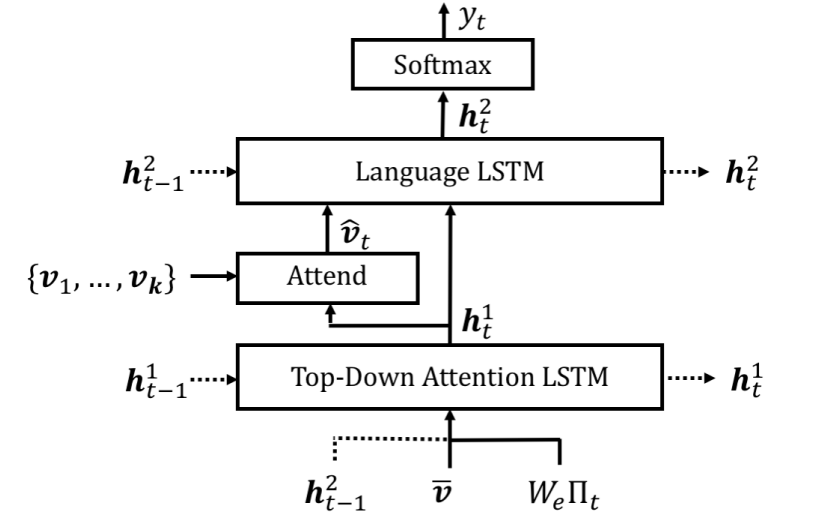
\includegraphics[width=0.75\textwidth]{topdown.png}
\end{figure}
\paragraph{Top-Down Attention LSTM}


Here is the input vector described for the Attention LSTM. 
\begin{figure}[H]
\centering
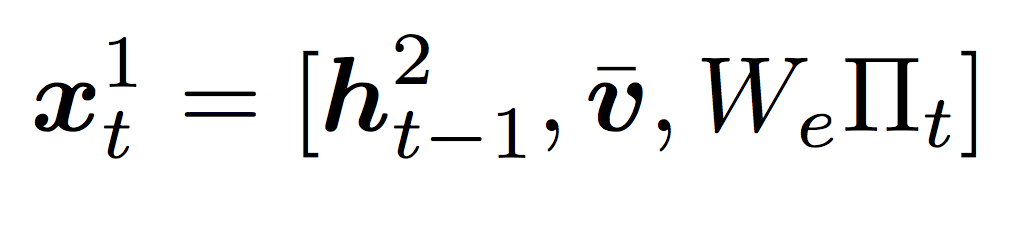
\includegraphics[width=0.25\textwidth]{b.png}
\end{figure}
\begin{figure}[H]
\centering
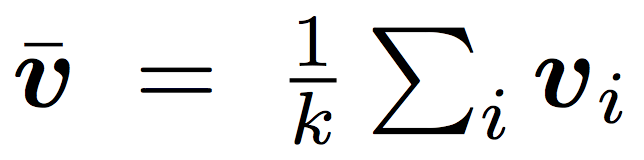
\includegraphics[width=0.15\textwidth]{a.png}
\end{figure}
\begin{figure}[H]
\centering
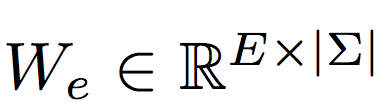
\includegraphics[width=0.15\textwidth]{c.png}
\end{figure}
$h_t2$ is the output of the language LSTM, $v_i$ is the mean-pooled image feature, and W is a word embedding matrix $\Sigma$, and $\Pi_t$ is one-hot encoding of the input word
at timestep $t$.
\\
\noindent 
The attention LSTM thus is provided with more than adequate information regarding the state of the language LSTM, the image features, and the partial caption.

Given the output $h_t^1$ of the attention LSTM, a normalized attention weight is calculated $\alpha_i,t$ for
each $k$ image feature $v_i$ as follows:

\begin{figure}[H]
\centering
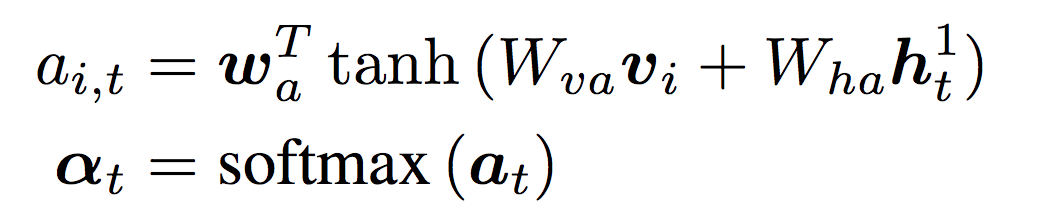
\includegraphics[width=0.4\textwidth]{d.png}
\end{figure}

\noindent where:

\begin{figure}[H]
\centering
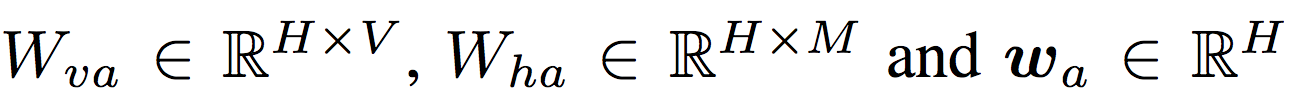
\includegraphics[width=0.5\textwidth]{e.png}
\end{figure}

\noindent are
learned parameters. The attended feature  input
to the language LSTM is a culmination of all input features:
\begin{figure}[H]
\centering
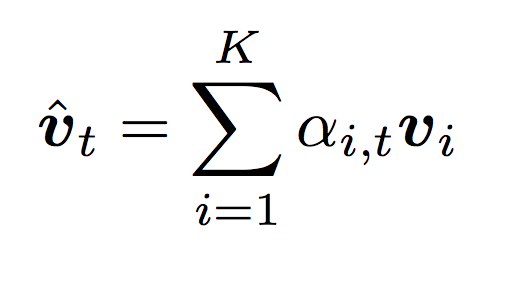
\includegraphics[width=0.2\textwidth]{f.png}
\end{figure}

\paragraph{Language LSTM}
The input to the language model LSTM consists of the attended image feature, and the output of the attention LSTM.
\begin{figure}[H]
\centering
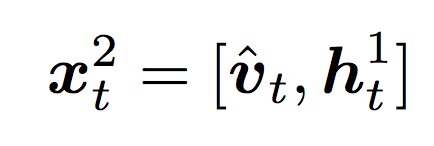
\includegraphics[width=0.15\textwidth]{g.png}
\end{figure}
$y_1:T$ to refers to a sequence of words
$(y_1, ..., y_T )$. The conditional distribution
over possible output words is given by:
\begin{figure}[H]
\centering
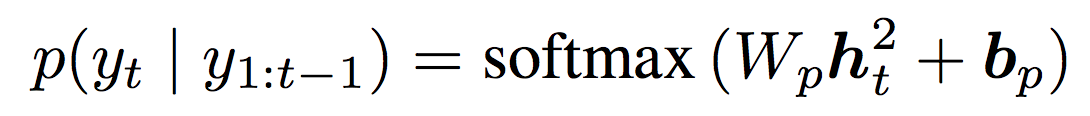
\includegraphics[width=0.4\textwidth]{h.png}
\end{figure}

where
\begin{figure}[H]
\centering
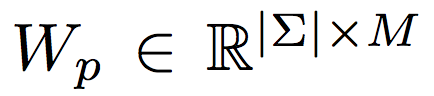
\includegraphics[width=0.15\textwidth]{i.png}
\end{figure}
and 
\begin{figure}[H]
\centering
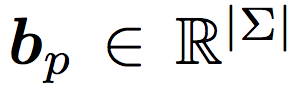
\includegraphics[width=0.10\textwidth]{j.png}
\end{figure}

\noindent are weights and biases. The distribution over complete output sequences is calculated as the product of conditional distributions:

\begin{figure}[H]
\centering
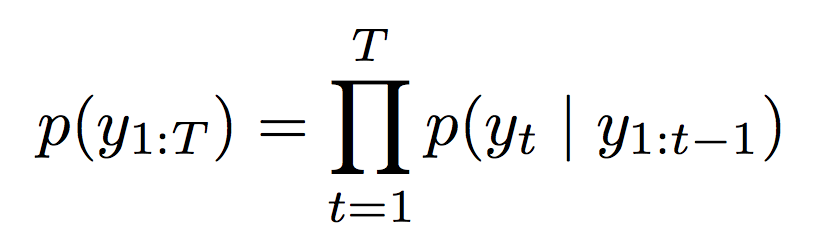
\includegraphics[width=0.35\textwidth]{k.png}
\end{figure}

\paragraph{Objective}
Given a target ground truth sequence $y
_1:T^∗$ and a captioning model with parameters $\theta$, we minimize the following cross entropy loss:

\begin{figure}[H]
\centering
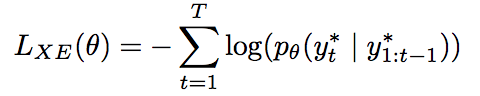
\includegraphics[width=0.4\textwidth]{l.png}
\end{figure}

\begin{figure}[H]
\centering
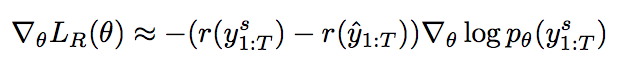
\includegraphics[width=0.5\textwidth]{n.png}
\end{figure}
\cite{DBLP:journals/corr/AndersonHBTJGZ17}

\section{Dataset}
We are using one of the most widely used dataset for image captioning tasks. The Flickr8k data set contains images found of Flickr. There are 8k images with associated captions. Each image in the dataset contains 5 captions. Each of the five captions describes the image in a different way, with different grammar and verbs. Out of the 8000 images, 7000 are used for training the model. The remaining images are utilized for testing the performance of the model with an associated bleu score. \par
We chose to use the Flickr8k because it is smaller in size, and faster to train. You may use this model on other benchmark datasets as well namely, Flickr30k and MSCOCO

\section{Evaluation}
\subsection{Metrics}

Evaluation is done on the standard metrics which are as follows: CIDEr \cite{DBLP:journals/corr/VedantamZP14a}, BLEU \cite{papineni2002bleu},    ROUGE-L \cite{lin2004rouge}, METEOR \cite{denkowski2014meteor}, SPICE \cite{DBLP:journals/corr/AndersonFJG16}

\begin{figure}[H]
\centering
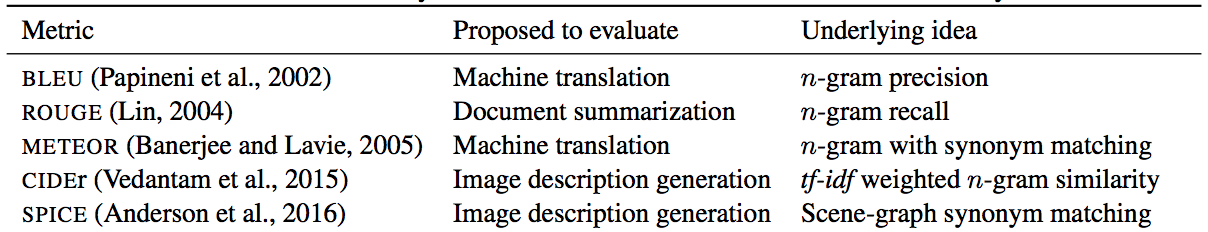
\includegraphics[width=1\textwidth]{metrics.png}
\caption{\label{fig:arch}Summary of metrics for automatic evaluation of generated captions}
\end{figure}

\subsubsection{BLEU}
BLEU (Papineni et al., 2002) is one of the first metrics
that have been in use for measuring similarity
between two sentences. It has been initially proposed
for machine translation, and defined as the
geometric mean of n-gram precision scores multiplied
by a brevity penalty for short sentences. In
our experiments, we use the smoothed version of
BLEU as described in (Lin and Och, 2004).
\subsubsection{METEOR}
METEOR (Banerjee and Lavie, 2005) is another
machine translation metric. It is defined as the
harmonic mean of precision and recall of unigram
matches between sentences. Additionally, it
makes use of synonyms and paraphrase matching.
METEOR addresses several deficiencies of BLEU
such as recall evaluation and the lack of explicit
word matching. n-gram based measures work reasonably
well when there is a significant overlap between reference and candidate sentences; however
they fail to spot semantic similarity when
the common words are scarce. METEOR handles
this issue to some extent using WordNet-based
synonym matching, however just looking at synonyms
may be too restrictive to capture overall semantic
similarity.
\subsubsection{SPICE}
Another recently proposed metric for evaluating
image caption similarity is SPICE (Anderson et al.,
2016). It is based on the agreement of the scenegraph
tuples (Johnson et al., 2015; Schuster et al.,
2015) of the candidate sentence and all reference
sentences. Scene-graph is essentially a semantic
representation that parses the given sentence to semantic
tokens such as object classes C, relation
types R and attribute types A. Formally, a candidate
caption c is parsed into a scene-graph as
G(c) = hO(c), E(c), K(c)i
where G(c) denotes the scene graph of caption c,
O(c) ⊆ C is the set of object mentions, E(c) ⊆
O(c) × R × O(c) is the set of hyper-edges representing
relations between objects, and K(c) ⊆
O(c) × A is the set of attributes associated with
objects. Once the parsing is done, a set of tuples is formed by using the elements of G and their possible
combinations. SPICE score is then defined as
the F1-score based on the agreement between the
candidate and reference caption tuples. For tuple
matching, SPICE uses WordNet synonym matching
(Pedersen et al., 2004) as in METEOR (Banerjee
and Lavie, 2005). One problem is that the performance
becomes quite dependent on the quality
of the parsing. Figure 1 illustrates an example case
of failure. Here, swimming is parsed as an object,
with all its relations, and dog is parsed as an attribute.
\subsubsection{CIDEr}
CIDEr (Vedantam et al., 2015) is a recent metric
proposed for evaluating the quality of image
descriptions. It measures the consensus between
candidate image description ci and the reference
sentences, which is a set Si = {si1, . . . , sim} provided
by human annotators. For calculating this
metric, an initial stemming is applied and each
sentence is represented with a set of 1-4 grams.
Then, the co-occurrences of n-grams in the reference
sentences and candidate sentence are calculated.
In CIDEr, similar to tf-idf, the n-grams that
are common in all image descriptions are downweighted.
Finally, the cosine similarity between
n-grams (referred as CIDErn) of the candidate and
the references is computed.
CIDEr is designed as a specialized metric for
image captioning evaluation, however, it works in
a purely linguistic manner, and only extends existing
metrics with tf-idf weighting over n-grams.
This sometimes causes unimportant details of a
sentence to be weighted more, resulting in a relatively
ineffective caption evaluation.
\subsubsection{ROUGE}
ROUGE (Lin, 2004) is initially proposed for evaluation
of summarization systems, and this evaluation
is done via comparing overlapping n-grams,
word sequences and word pairs. In this study, we
use ROUGE-L version, which basically measures
the longest common subsequences between a pair
of sentences. Since ROUGE metric relies highly
on recall, it favors long sentences, as also noted
by (Vedantam et al., 2015).

\subsection{Feature	Extraction}
For feature extraction we used ResNet\cite{DBLP:journals/corr/HeZRS15} that was pre-trained on ImageNet\cite{deng2009imagenet}, before feeding these features to the caption generation models. ResNet CNN is run on the original image and the last convolution layer feature is adaptively average pool to fixed size.

\begin{figure}[H]
\centering
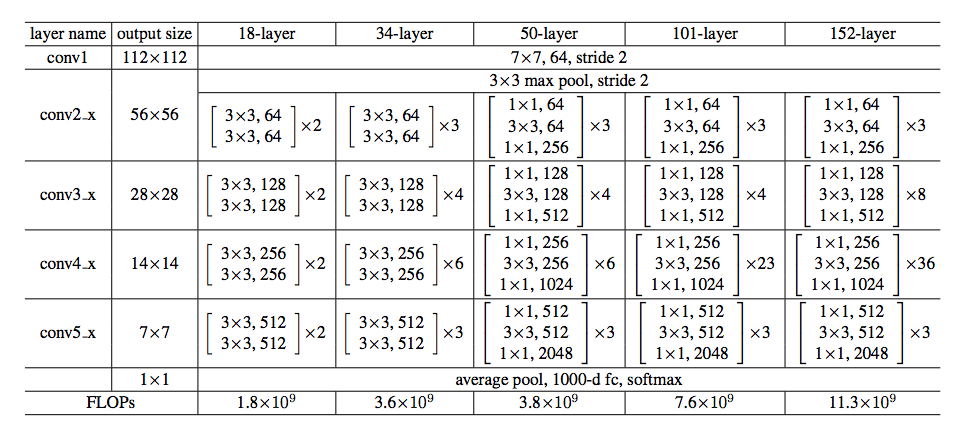
\includegraphics[width=1\textwidth]{resnet.png}
\caption{\label{fig:arch}Diagram representing the ResNet architecture.}
\end{figure}

\subsection{Experiment Setup}

All variants of our models were trained with stochastic gradient descent using adaptive learning rate Adam\cite{kingma2014adam}. We used a batch size of $10$, learning rate $5 X 10^-4$ with 0 start weight decay, trained for 25 epochs, which took over an hour for the Top Down Network but only few minutes for Show Tell and Show Attend and Tell owning to their reduced complexity on a TITAN X GPU.\\
\noindent We used pretrained ResNet-101, on the ImageNet dataset as a starting point for feature extraction for all our experiments.\\
\noindent An extremely fast implementation of R-CNN is used, so called Fast R-CNN\cite{ren2015faster} for the Top Down Network.\\
\noindent For the Show, Attend and Tell model we used the soft attention mechanism only, the hard attention mechanism is considerably more complex when it comes to actual implementation due to its stochastic training procedure.

\subsection{Results}

Each of these tables compares the results given in the respective paper in comparison to the results we achieved during our experiments. As mentioned the Flickr8k dataset is usually divided into 6000 for training, 1000 for development and 1000 for testing. The evaluation scores usually come from the 1000 test images that are segregated. 
The standard papaer of Top-Down Bottom-up attention evaluates on the MSCOCO dataset.The Show and Tell , and Show, Attend and Tell official paper does evaluation on all three benchmark datasets. 
\subsubsection{Show and Tell Model results}
\begin{center}
 \begin{tabular}{|c| c| c| c| c| c| c | c| c| c|} 
 \hline
 
 Paper Details & BLEU1 & BLEU2 & BLEU3 & BLEU4 & CIDEr & ROUGE-L & METEOR & SPICE\\ [0.2ex] 
 \hline
  Standard paper & 0.63 & 0.41 & 0.27 & - & - & - & - & - & \\ 
 \hline
\textbf{Ours} & 0.613& 0.433& 0.301& 0.209 & 0.491 &0.462&0.199&0.135&  \\
 \hline

\hline
\end{tabular}
\end{center}
\subsubsection{Show Attend and Tell results}
\begin{center}
 \begin{tabular}{|c| c| c| c| c| c| c | c| c| c|} 
 \hline
 
 Paper Details & BLEU1 & BLEU2 & BLEU3 & BLEU4 & CIDEr & ROUGE-L & METEOR & SPICE\\ [0.2ex] 
 \hline
  Standard paper & 0.67 & 0.448 & 0.299 & 0.195 & - & - & 0.195 & - & \\ 
 \hline
\textbf{Ours} & 0.652& 0.473& 0.332& 0.228 & 0.600 &0.483&0.216&0.157&  \\
 \hline

\hline
\end{tabular}
\end{center}
\subsubsection{Bottom up and Top Down Model results}

\begin{center}
 \begin{tabular}{|c| c| c| c| c| c| c | c| c| c|} 
 \hline
 
 Paper Details & BLEU1 & BLEU2 & BLEU3 & BLEU4 & CIDEr & ROUGE-L & METEOR & SPICE\\ [0.2ex] 
 \hline
  Standard paper & 0.772 & - & - & 0.362 & 113.5(denorm) & 0.564 & 0.270 & 0.203& \\ 
 \hline
\textbf{Ours} & 0.657& 0.477& 0.334& 0.230 & 0.59 & 0.48& 0.21& -&  \\
 \hline

\end{tabular}
\end{center}


\section{Conclusion}
On conclusion we would like to mention that, here we evaluate three major architectures and present evaluation on various matrices which are state of the art and compare it to the evaluation results given in the official paper of these architectures. Firstly, we present and evaluate show and tell model which combines state of the art language language and vision model. Secondly we evaluate Show, attention and tell model which is an attention based approach, its unique in the sense that this architecture the learned alignments correspond very well to the human intuition. Thirdly we evaluate the novel implementation of bottom up and top down together which allows attention to be calculated at the low level of objects and other salient features. This paper is a one-stop evaluation shelf for the three popular architectures in Image Captioning.
\\
\noindent
Here are some sample image caption results:
\\
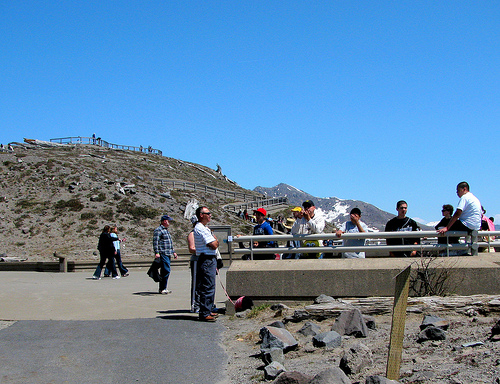
\includegraphics[width=\textwidth]{3562050678_4196a7fff3.jpg}
\\
\begin{center}
 \begin{tabular}{|c| c| c| c| c| c| c | c| c| c|} 
 \hline
 
 Ground Truth & tourists are standing a mountain viewpoint beneath a clear blue sky\\ [0.2ex] 
 \hline
  Show and Tell & a group of people are sitting on a bench in front of the ocean\\ 
 \hline
	Show, Attend, and Tell & a group of people are sitting on a bench\\
 \hline
  Top Down / Bottom Up & a group of people are sitting on a rocky hill\\ 
 \hline
\end{tabular}
\end{center}

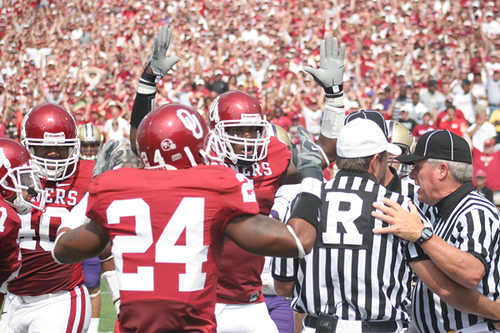
\includegraphics[width=\textwidth]{241347204_007d83e252.jpg}
\\
\begin{center}
 \begin{tabular}{|c| c| c| c| c| c| c | c| c| c|} 
 \hline
 
 Ground Truth & A football player in red and white is holding both hands up\\ [0.2ex] 
 \hline
  Show and Tell & a football player in a red jersey is running\\ 
 \hline
	Show, Attend, and Tell & a football player in red is being tackled\\
 \hline
  Top Down / Bottom Up & a group of football players in red and white uniforms\\ 
 \hline
\end{tabular}
\end{center}
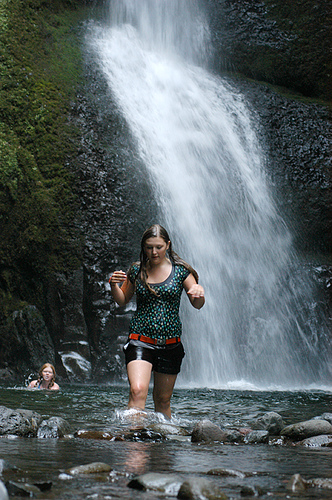
\includegraphics[width=\textwidth]{219301555_17883a51bd.jpg}
\\
\begin{center}
 \begin{tabular}{|c| c| c| c| c| c| c | c| c| c|} 
 \hline
 
 Ground Truth & A woman wading through a pool in front of a waterfall\\ [0.2ex] 
 \hline
  Show and Tell & a woman in a bikini is standing on a rock overlooking the ocean\\ 
 \hline
	Show, Attend, and Tell &  a girl in a swimsuit is standing in the water\\
 \hline
  Top Down / Bottom Up & a girl in a swimsuit is splashing in the water\\ 
 \hline
\end{tabular}
\end{center}
\section{Team Roles}
Dan and Saurabh were responsible for the Top down Bottom Up and Show, Attend and Tell models, respectively. While Robin was responsible for the Show and Tell model. Robin was in charge of acquiring the Flickr8K dataset. Quite some time was spent together as a team figuring out how to get the input and evaluation for the generic model working first. Saurabh and Robin worked on the paper tried to come up with proper explanation and neatly present it while Dan worked on the power-point presentation and was responsible for the attachment of the pictures in the paper.

\section{Future Work}
As far as future work is concerned we have just implemented using the smallest benchmark dataset Flickr8k. There is high possibility of hyper-tuning as well. We did our experiments with 25 epochs and a particular learning rate. There is scope to try out a different dataset such as Flickr30k or MSCOCO or any other as seem fit with proper tuning, learning rate and change of other hyperparameters.

\bibliographystyle{plain}
\bibliography{sample.bib}

\end{document}

